\SourcePage{417}{420}
\section{Predissociation}

The theory of diatomic molecules developed in this chapter rests chiefly on the assumption that a molecule's wave function can be separated into the product of an electronic wave function (in which the internuclear distance enters as a parameter) and a wave function describing the motion of the nuclei. Equivalently, certain small terms that couple the nuclear and electronic motions are omitted from the exact molecular Hamiltonian.

When these terms are included perturbatively, transitions arise between different electronic states. The transitions of greatest physical importance are those for which at least one of the states belongs to the continuous spectrum.

Figure~30 shows the potential-energy curves of two electronic terms (more precisely, the effective potential energy $U_J$ for the specified rotational states of the molecule). The energy $E'$ belongs to a particular vibrational level of a stable molecule in electronic state 2. In state 1, the same energy is in the continuous-spectrum region. Thus a transition from state 2 to state 1 causes the molecule to decay spontaneously; this phenomenon is called \emph{predissociation}\footnote{Curve 1 need not have a minimum at all when it represents purely repulsive forces between the atoms.}. Consequently, the discrete-spectrum state represented by curve 2 actually has a finite lifetime. The discrete

\begin{figure}[ht]
\centering
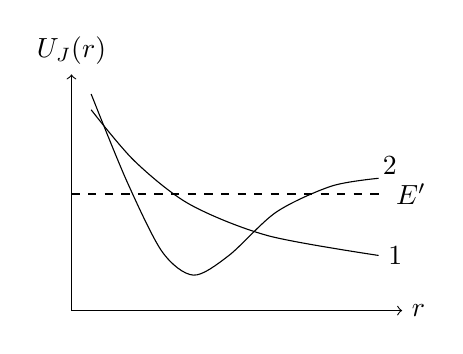
\begin{tikzpicture}[x=1cm,y=1cm]
\draw[->] (0,0)--(4.2,0) node[right]{$r$}; \draw[->] (0,0)--(0,3) node[above]{$U_J(r)$};
\draw[smooth] plot coordinates {(.25,2.55)(.8,1.9)(1.5,1.35)(2.5,.95)(3.9,.7)} node[right]{1};
\draw[smooth] plot coordinates {(.25,2.75)(.7,1.65)(1.15,.75)(1.55,.45)(2,.7)(2.6,1.25)(3.3,1.58)(3.9,1.68)} node[above right=-2pt]{2};
\draw[dashed] (0,1.48)--(4,1.48) node[right]{$E'$};
\end{tikzpicture}
\caption*{Fig. 30}
\end{figure}

\SourcePage{418}{421}
energy level is therefore broadened: it acquires a certain width (see the end of \S~44).

If the total energy $E$ lies above the dissociation threshold in both states, a transition from one state to the other represents what is known as a \emph{collision of the second kind}. For example, in a $1\to2$ transition two atoms collide, enter excited states, and separate with reduced kinetic energy (as $r\to\infty$, curve 1 lies below curve 2; the difference $U_2(\infty)-U_1(\infty)$ is the atoms' excitation energy).

Because the nuclei are very massive, their motion is semiclassical. Determining the probability of the transitions under discussion is therefore a problem of the class considered in \S~52. The general arguments given there show that the transition probability is controlled by a point at which the transition could occur classically\footnote{Alternatively, it may be the point $r=0$, where the potential energy becomes infinite.}. Since the total energy of the two-atom system (the molecule) is conserved during such a transition, ``classical feasibility'' requires equality of the effective potential energies: $U_{J1}(r)=U_{J2}(r)$. The molecule's total angular momentum is conserved as well, so the centrifugal energies are identical in the two states. The stated condition consequently reduces to equality of the potential energies,
\begin{equation}U_1(r)=U_2(r),\tag{90.1}\end{equation}
and contains no angular-momentum quantity whatever.

If equation (90.1) has no real roots in the classically accessible region (the region where $E>U_{J1},U_{J2}$), then, according to \S~52, the transition probability is exponentially small\footnote{A special situation arises when a transition involves a molecular term obtainable from two distinct pairs of atomic states (see the end of \S~85), that is, when the potential-energy curve seems to divide into two branches toward increasing separations.  In this situation the transition probability increases substantially; for an example, see A.~I.~Voronin, E.~E.~Nikitin~// Optika i spektr. 1968. Vol.~25. P.~803.}

.
Transitions have an appreciable probability only when the potential-energy curves intersect within the classically accessible region (as shown in Fig.~30).

In that event the exponent in formula (52.1) vanishes (so that this formula is, of course, inapplicable), and the transition probability is consequently given by a nonexponential expression (to be derived below).

Condition (90.1) can


\SourcePage{419}{422}
then be interpreted visually as follows. Equal potential (and total) energies also imply equal momenta. Thus, in place of (90.1), one may write
\begin{equation}r_1=r_2,\qquad p_1=p_2,\tag{90.2}\end{equation}
where $p$ is the momentum of the relative radial motion of the nuclei, while the subscripts 1 and 2 refer to the two electronic states. Thus, at the instant of transition, the separation and momentum of the nuclei may be said to remain unchanged (the so-called \emph{Franck--Condon principle}). Physically, this follows because electronic velocities are large in comparison with nuclear velocities, and ``during the electronic transition'' the nuclei have no time to change their positions and velocities appreciably.


The selection rules for these transitions are readily established. First, there are two evident exact rules: neither the total angular momentum $J$ nor the sign of the term (positive or negative; see \S~86) may change in a transition. This follows directly because conservation of total angular momentum and invariance of the wave-function character under inversion of the coordinate system are exact laws for every closed system of particles.

There is also, to high accuracy, a rule forbidding transitions between states of different parity in a molecule made of identical atoms. Indeed, a state's parity is fixed uniquely by the nuclear spin and the term sign. Conservation of the term sign is exact, while nuclear spin is conserved to high accuracy because its interaction with the electrons is weak.

The existence of an intersection of the potential-energy curves requires terms of different symmetry (see \S~79). Consider transitions that occur already in first-order perturbation theory. We first note that the Hamiltonian terms producing these transitions are precisely those responsible for the $\Lambda$-doubling of levels. Foremost among them are the terms describing spin--orbit interaction. Each is a product of two axial vectors, one of spin character and the other of coordinate character; these vectors, it should be stressed, are by no means simply $\widehat{\mathbf S}$ and $\widehat{\mathbf L}$. They consequently have nonzero matrix elements for transitions in which $S$ and $\Lambda$ change by $0,\pm1$.

\SourcePage{420}{423}
The case in which $\Delta S=\Delta\Lambda=0$ simultaneously (with $\Lambda\ne0$) must be excluded, since the symmetry of the term would then remain entirely unchanged in the transition.

A transition between two $\Sigma$ terms is possible only if their superscripts have opposite signs, one being $\Sigma^+$ and the other $\Sigma^-$ (an axial vector has matrix elements only for transitions between $\Sigma^+$ and $\Sigma^-$; see \S~87).


The Hamiltonian contains a term describing the coupling between molecular rotation and the orbital angular momentum. This term is proportional to $\widehat{\mathbf J}\mathbin{\cdot}\widehat{\mathbf L}$, and its matrix elements are nonzero for transitions with $\Delta\Lambda=\pm1$ and no change of spin. (For $\Delta\Lambda=0$, matrix elements occur only for the $\zeta$ component of the vector, i.e. $L_\zeta$; however, $L_\zeta$ is diagonal in the electronic states.)


Besides the terms just considered, a further perturbation arises because the nuclear kinetic-energy operator acts not only upon the nuclear wave function, but also upon the electronic function that depends parametrically on $r$. The corresponding Hamiltonian terms have the same symmetry as the unperturbed Hamiltonian. They can therefore produce transitions only between electronic terms of identical symmetry; the probability of these transitions is negligible because the terms do not intersect.

We now calculate the transition probability explicitly, taking a collision of the second kind for definiteness. By the general formula (43.1), the required probability is
\begin{equation}w=\frac{4\pi^2}{\hbar^2}\left|\int\chi_{\text{nuc},2}V(r)\chi_{\text{nuc},1}\,dr\right|^2,\tag{90.3}\end{equation}
where $\chi_{\text{nuc}}=r\psi_{\text{nuc}}$ and $V(r)$ is the perturbing energy. The final wave function $\chi_{\text{nuc},2}$ must be normalized to a delta-function of the energy. With this normalization, the semiclassical function is
\begin{equation}\chi_{\text{nuc},2}=\sqrt{\frac2{\pi\hbar v_2}}\cos\left(\frac1\hbar\int_{a_2}^r p_2,dr-\frac\pi4\right).\tag{90.4}\end{equation}
For the initial state we write

\SourcePage{421}{424}
\begin{equation}\chi_{\text{nuc},1}=\frac2{\sqrt{v_1}}\cos\left(\frac1\hbar\int_{a_1}^r p_1,dr-\frac\pi4\right).\tag{90.5}\end{equation}
It is normalized so that each of the two travelling waves carries unit current density. Substitution of these functions in (90.3) gives a dimensionless transition probability $w$, interpretable as the probability accumulated when the nuclei pass the point $r=r_0$ twice.

The matrix element contains a product of cosines, which we resolve into cosines of the sum and difference of their arguments. Near $r=r_0$ only the latter cosine is relevant, and hence
\[
w=\frac4{\hbar^2}\left|\int\frac{V(r)}{\sqrt{v_1v_2}}\cos\left(\frac1\hbar\int_{a_1}^r p_1dr-\frac1\hbar\int_{a_2}^r p_2dr\right)dr\right|^2.
\]
The integral converges rapidly away from the intersection. Expanding the argument in powers of $\xi=r-r_0$ and using $p_1=p_2$ at the intersection, we find
\[
\int^r p_1dr-\int^r p_2dr\approx S_0+\frac12\left(\frac{dp_1}{dr}-\frac{dp_2}{dr}\right)_0\xi^2.
\]
Differentiation of $p_1^2/2\mu+U_1=p_2^2/2\mu+U_2$ gives
\[
v_1\frac{dp_1}{dr}-v_2\frac{dp_2}{dr}=F_1-F_2,
\]

\SourcePage{422}{425}
and consequently
\[
\int^r p_1dr-\int^r p_2dr\approx S_0+\frac{F_1-F_2}{2v}\xi^2.
\]
Use of the familiar integral then yields
\begin{equation}w=\frac{8\pi V^2}{\hbar v|F_2-F_1|}\cos^2\left(\frac{S_0}{\hbar}+\frac\pi4\right).\tag{90.6}\end{equation}
The quantity $S_0/\hbar$ is large and varies rapidly with energy. On averaging, the squared cosine is replaced by its mean, giving
\begin{equation}w=\frac{4\pi V^2}{\hbar v|F_2-F_1|}.\tag{90.7}\end{equation}
(L.~D.~Landau, 1932). Every quantity on the right is evaluated at the intersection.

For predissociation, the decay probability per unit time is obtained by multiplying $w$ by $\omega/2\pi$:
\begin{equation}\frac1\tau=\frac{2\omega V^2}{\hbar v|F_2-F_1|}.\tag{90.8}\end{equation}

In referring to an intersection of terms, we have meant the eigenvalues of the unperturbed Hamiltonian $\widehat H_0$, excluding the terms $\widehat V$ that produce transitions. Once those terms are included, the intersection disappears and the curves separate as shown in Fig.~31.

\SourcePage{423}{426}
Let $U_{J1}(r)$ and $U_{J2}(r)$ be two eigenvalues of $\widehat H_0$. The method of \S~79 gives
\begin{equation}U_{b,a}(r)=\frac12(U_{J1}+U_{J2})\pm\frac12\sqrt{(U_{J1}-U_{J2})^2+4V^2}.\tag{90.9}\end{equation}
The separation of the levels is
\begin{equation}\Delta U=\sqrt{(U_{J1}-U_{J2})^2+4V^2},\tag{90.10}\end{equation}
and its minimum value at $r=r_0$ is
\begin{equation}(\Delta U)_{\min}=2|V(r_0)|.\tag{90.11}\end{equation}
Near this point,
\begin{equation}\Delta U=\sqrt{(F_2-F_1)^2(r-r_0)^2+4V^2}.\tag{90.12}\end{equation}

\begin{figure}[ht]
\centering
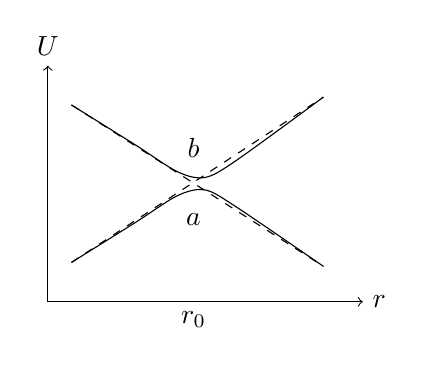
\begin{tikzpicture}[x=1cm,y=1cm]
\draw[->] (0,0)--(4,0) node[right]{$r$}; \draw[->] (0,0)--(0,3) node[above]{$U$};
\draw[dashed] (.3,.5)--(3.5,2.6); \draw[dashed] (.3,2.5)--(3.5,.45);
\draw[smooth] plot coordinates {(.3,2.5)(1.1,2)(1.65,1.65)(2,1.58)(2.4,1.8)(3.5,2.6)};
\draw[smooth] plot coordinates {(.3,.5)(1.1,1)(1.65,1.35)(2,1.42)(2.4,1.2)(3.5,.45)};
\node at (1.85,1.95){$b$}; \node at (1.85,1.05){$a$}; \node[below] at (1.85,0){$r_0$};
\end{tikzpicture}
\caption*{Fig. 31}
\end{figure}

These formulas require $(\Delta U)_{\min}$ to be small compared with the distance to the other terms. If condition (90.19) is not satisfied, ordinary perturbation theory cannot be used for the transition probability, and a more general treatment is needed.

\SourcePage{424}{427}
In the neighborhood of the intersection, we treat the nuclear motion semiclassically, replace the velocity operator by the constant $v$, and put $\xi=r-r_0=vt$. The problem reduces to
\begin{equation}i\hbar\frac{\partial\Psi}{\partial t}=[\widehat H_0(t)+\widehat V(t)]\Psi.\tag{90.13}\end{equation}
Let $\psi_a$ and $\psi_b$ denote the electronic states associated with curves $a$ and $b$. We seek a solution of the form
\begin{equation}\Psi=a(t)\psi_a+b(t)\psi_b.\tag{90.14}\end{equation}
Under the boundary condition $a=1,b=0$ as $t\to-\infty$, the quantity $|b(\infty)|^2$ is the probability of transition from curve $a$ to curve $b$ in a single passage through the point. During a double passage, the transition can follow either $a\to b\to b$ or $a\to a\to b$; thus
\begin{equation}w=2|b(\infty)|^2[1-|b(\infty)|^2].\tag{90.15}\end{equation}

The value of $b(\infty)$ can be found by the method of \S~53\footnote{In \S~53 the entire process was assumed to be adiabatic. Here adiabaticity may fail immediately around $r_0$; only adiabatic behavior at large $|t|$ and the possibility of retaining just two levels are essential.}.

\SourcePage{425}{428}
The curves $U_a(t)$ and $U_b(t)$ intersect at the imaginary points
\begin{equation}t_0^{(\pm)}=\pm i\frac{2V}{|F_2-F_1|v}=\pm i\tau_0.\tag{90.16}\end{equation}
Passing into the complex $t$ plane and going around the point $t_0^{(+)}$, we use
\begin{equation}\Delta U=\sqrt{(F_2-F_1)^2v^2t^2+4V^2}\tag{90.17}\end{equation}
to obtain finally
\begin{equation}w=2\exp\left(-\frac{2\pi V^2}{\hbar v|F_2-F_1|}\right)\left[1-\exp\left(-\frac{2\pi V^2}{\hbar v|F_2-F_1|}\right)\right].\tag{90.18}\end{equation}
(C.~Zener, 1932). The probability is small in either limiting case. When $V^2\gg\hbar v|F_2-F_1|$, it is

\SourcePage{426}{429}
exponentially small (the adiabatic case); when
\begin{equation}V^2\ll\hbar v|F_2-F_1|\tag{90.19}\end{equation}
formula (90.18) reduces to (90.7). Equation (90.17) shows that $\tau\sim|V|/(|F_2-F_1|v)$ is the ``nuclear transit time'' past the intersection.

Finally, consider the phenomenon related to predissociation that is known as perturbations in the spectrum of diatomic molecules. If two discrete molecular levels $E_1,E_2$ are close, the possibility of a transition shifts them. According to (79.4),
\begin{equation}E=\frac{E_1+E_2}{2}\pm\sqrt{\left(\frac{E_1-E_2}{2}\right)^2+|V_{12}^{\text{nuc}}|^2}.\tag{90.20}\end{equation}
The levels move apart, by an amount that increases as $|E_1-E_2|$ decreases. The matrix element $V_{12}^{\text{nuc}}$ is calculated as above, except that the discrete-spectrum nuclear functions are normalized to unity. Comparison gives
\begin{equation}|V_{12}^{\text{nuc}}|^2=w\frac{\hbar\omega_1}{2\pi}\frac{\hbar\omega_2}{2\pi}.\tag{90.21}\end{equation}

\SourcePage{427}{430}
\ProblemHeading 1. Calculate the total cross section for second-kind collisions, as a function of the kinetic energy $E$ of the colliding atoms, for transitions produced by spin--orbit interaction (L.~D.~Landau, 1932).


\SolutionHeading Since the nuclear motion is semiclassical, an impact parameter $\rho$ may be introduced and we may set $d\sigma=2\pi\rho,d\rho,w(\rho)$. For spin--orbit interaction, the matrix element $V(r)$ is independent of the angular momentum. The velocity at the intersection is
\[
v=\sqrt{\frac2\mu\left(E-U-\frac{\rho^2E}{r_0^2}\right)}.
\]
Integration over $\rho$ gives
\[
\sigma=\frac{4\sqrt{2\mu}\pi^2V^2r_0^2}{\hbar|F_2-F_1|}\frac{\sqrt{E-U}}{E}.
\]

\ProblemHeading 2. Do the same for transitions caused by the coupling of molecular rotation to orbital angular momentum (L.~D.~Landau, 1932).

\SolutionHeading The matrix element has the form $V(r)=MD/\mu r^2$, where $D(r)$ is the matrix element of the electronic orbital angular momentum. The same method gives
\[
\sigma=\frac{16\sqrt2\pi^2D^2(E-U)^{3/2}}{3\hbar\mu r_0^2|F_2-F_1|E}.
\]

\ProblemHeading 3. Find the transition probability for energies $E$ close to the potential energy $U$ at the intersection.

\SolutionHeading For small $E-U$, formula (90.7) is inapplicable. Near the intersection, replace the curves by straight lines $U_1=U-F_1\xi$, $U_2=U-F_2\xi$, where $\xi=r-r_0$. The wave functions are those for one-dimensional motion in a uniform field. Calculation in the momentum representation gives

\SourcePage{428}{431}
\begin{equation}
w=\frac{4\pi V^2(2\mu)^{2/3}}{\hbar^{4/3}(F_1F_2)^{1/2}(F_2-F_1)^{2/3}}
\Phi^2\!\left[-\frac{E-U}{\hbar^{2/3}}\left(\frac{2\mu(F_2-F_1)^2}{F_1^2F_2^2}\right)^{1/3}\right],
\tag{90.22}
\end{equation}
where $\Phi$ is the Airy function (see \S~b of the Mathematical Supplements). For large $E-U$, this formula reduces to (90.7).

\ProblemHeading 4. Find the charge-transfer probability in a distant, slow ($v\ll1$) collision between a hydrogen atom and a proton (O.~V.~Firsov, 1951)\footnote{Atomic units are used in this problem.}.

\SolutionHeading Regard the system $\mathrm H+\mathrm H^+$ as a hydrogen molecular ion (see the problem in \S~81). Charge transfer consists in moving the electron from the state $\psi_1$, localized at the first nucleus, to the state $\psi_2$ near the second. The stationary states are
\[
\psi_{g,u}=\frac1{\sqrt2}(\psi_1\pm\psi_2).
\]
Their energies are $U_{g,u}(R)$. For the specified slow classical motion of the nuclei, the time dependence is supplied by the factors $\exp[-i\int U_{g,u}(t)dt]$. As $t\to\infty$, the charge-transfer probability is
\[
w=\sin^2\eta,\qquad \eta=\frac12\int_{-\infty}^{\infty}(U_u-U_g)dt.
\]
At large impact parameters $\rho$, put $R=\sqrt{\rho^2+v^2t^2}$ and use formula (4) of the problem in \S~81:
\[
\eta=\frac4v\int_\rho^\infty\frac{R^2e^{-R-1}}{\sqrt{R^2-\rho^2}},dR.
\]
For $\rho\gg1$, putting $R=\rho(1+x)$ gives
\[
\eta=\frac{2\sqrt{2\pi}}{ev}\rho^{3/2}e^{-\rho}.
\]
